\section{Lessons Learned Perspective}
\subsection{Monitoring} \label{section:llmonitoring}
Monitoring proved very useful, and especially monitoring the response time of various endpoints allowed us to determine bottlenecks. This showed us one endpoint being significantly slower than the rest and allowed us to optimize the query, thereby decreasing response time from 25 seconds to 150ms, a 100x factor decrease.
\\
Due to the lack of infrastructure monitoring, identifying the state of our system was more complicated than necessary. Setting up infrastructure monitoring would have allowed us to get a quick and easy overview of the various containers' status. Instead, we were required to SSH into the different droplets to obtain this information. Furthermore, aggregating system information, such as CPU, RAM, and disk usage, from the droplets and database would have been beneficial. This would allow us to monitor the status on the server itself, thereby resulting in a single access point for all monitoring and logging. This could also be integrated with the previously mentioned alerts \ref{section:alerts}, which would allow us to react to potential threats, e.g. too high RAM or CPU usage.

\subsection{Reliant on GitHub Actions}
Due to our CI/CD pipeline being fully dependent on GitHub actions, we experienced a significant delay when this service was down. An example of this is shown below in figure \ref{fig:github-action-query}, where the workflow had been started and 17 minutes later still hasn't finished due to it being queued by GitHub.
\begin{figure}[H]
    \centering
    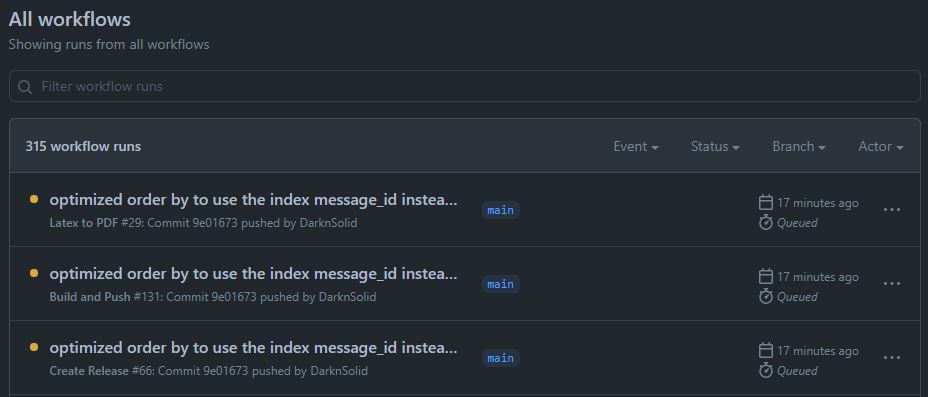
\includegraphics[width=1\linewidth]{report/images/github-actions-queue.png}
    \caption{Github action workflow queues}
    \label{fig:github-action-query}
\end{figure}


This could potentially be avoided by implementing a secondary backup pipeline with e.g. Travis or Vagrant or by having our own VM to run the CI/CD pipeline.

\subsection{Testing Environment}
Throughout the course, the importance of having a testing environment was learned.
When working with features not directly related to the code itself, such as GitHub actions, Docker, logging, etc. this was especially relevant.
Due to these features being dependent on a fully deployed system, they were not testable in a local environment.  
Furthermore, as these techniques were new to us, getting them to work (especially the CI/CD pipeline) often required a lot of testing which could result in downtime. Thereby, the testing environment would suffer from downtime rather than the production environment.
\\
An example of this was the implementation of logging. This required modifying various docker settings and installing plugins. Being able to test this in a development environment with no consequences made the process much easier.
An implementation of such an environment was attempted but did not work optimally due to various reasons. The most important was due to the fact that the simulator only made requests to the production environment. As testing many of our features required some activity on the server itself, it was difficult to see the actual impact of the changes made. This could have been resolved by running a similar simulator targeting the testing environment.

\subsection{Static Code Analysis}
We added ESLint late in the project after having refactored MiniTwit to the JavaScript framework. This revealed a large number of linting errors, which could have been avoided if linting was implemented from the start. Thereby the project could have started with fewer code smells and linting errors and the accumulation of technical debt throughout the first weeks could have been avoided.


\subsection{License}
We learned the importance of keeping track of the licenses used throughout a project. More specifically, we learned that to avoid a project being forced into being open-source you have to look out for libraries using copyleft licenses such as the GPL. 